% Options for packages loaded elsewhere
\PassOptionsToPackage{unicode}{hyperref}
\PassOptionsToPackage{hyphens}{url}
\PassOptionsToPackage{dvipsnames,svgnames,x11names}{xcolor}
%
\documentclass[
  11pt,
]{article}

\usepackage{amsmath,amssymb}
\usepackage{iftex}
\ifPDFTeX
  \usepackage[T1]{fontenc}
  \usepackage[utf8]{inputenc}
  \usepackage{textcomp} % provide euro and other symbols
\else % if luatex or xetex
  \usepackage{unicode-math}
  \defaultfontfeatures{Scale=MatchLowercase}
  \defaultfontfeatures[\rmfamily]{Ligatures=TeX,Scale=1}
\fi
\usepackage{lmodern}
\ifPDFTeX\else  
    % xetex/luatex font selection
    \setmainfont[]{Times New Roman}
\fi
% Use upquote if available, for straight quotes in verbatim environments
\IfFileExists{upquote.sty}{\usepackage{upquote}}{}
\IfFileExists{microtype.sty}{% use microtype if available
  \usepackage[]{microtype}
  \UseMicrotypeSet[protrusion]{basicmath} % disable protrusion for tt fonts
}{}
\makeatletter
\@ifundefined{KOMAClassName}{% if non-KOMA class
  \IfFileExists{parskip.sty}{%
    \usepackage{parskip}
  }{% else
    \setlength{\parindent}{0pt}
    \setlength{\parskip}{6pt plus 2pt minus 1pt}}
}{% if KOMA class
  \KOMAoptions{parskip=half}}
\makeatother
\usepackage{xcolor}
\usepackage[margin=2.5cm]{geometry}
\setlength{\emergencystretch}{3em} % prevent overfull lines
\setcounter{secnumdepth}{5}
% Make \paragraph and \subparagraph free-standing
\makeatletter
\ifx\paragraph\undefined\else
  \let\oldparagraph\paragraph
  \renewcommand{\paragraph}{
    \@ifstar
      \xxxParagraphStar
      \xxxParagraphNoStar
  }
  \newcommand{\xxxParagraphStar}[1]{\oldparagraph*{#1}\mbox{}}
  \newcommand{\xxxParagraphNoStar}[1]{\oldparagraph{#1}\mbox{}}
\fi
\ifx\subparagraph\undefined\else
  \let\oldsubparagraph\subparagraph
  \renewcommand{\subparagraph}{
    \@ifstar
      \xxxSubParagraphStar
      \xxxSubParagraphNoStar
  }
  \newcommand{\xxxSubParagraphStar}[1]{\oldsubparagraph*{#1}\mbox{}}
  \newcommand{\xxxSubParagraphNoStar}[1]{\oldsubparagraph{#1}\mbox{}}
\fi
\makeatother

\usepackage{color}
\usepackage{fancyvrb}
\newcommand{\VerbBar}{|}
\newcommand{\VERB}{\Verb[commandchars=\\\{\}]}
\DefineVerbatimEnvironment{Highlighting}{Verbatim}{commandchars=\\\{\}}
% Add ',fontsize=\small' for more characters per line
\usepackage{framed}
\definecolor{shadecolor}{RGB}{241,243,245}
\newenvironment{Shaded}{\begin{snugshade}}{\end{snugshade}}
\newcommand{\AlertTok}[1]{\textcolor[rgb]{0.68,0.00,0.00}{#1}}
\newcommand{\AnnotationTok}[1]{\textcolor[rgb]{0.37,0.37,0.37}{#1}}
\newcommand{\AttributeTok}[1]{\textcolor[rgb]{0.40,0.45,0.13}{#1}}
\newcommand{\BaseNTok}[1]{\textcolor[rgb]{0.68,0.00,0.00}{#1}}
\newcommand{\BuiltInTok}[1]{\textcolor[rgb]{0.00,0.23,0.31}{#1}}
\newcommand{\CharTok}[1]{\textcolor[rgb]{0.13,0.47,0.30}{#1}}
\newcommand{\CommentTok}[1]{\textcolor[rgb]{0.37,0.37,0.37}{#1}}
\newcommand{\CommentVarTok}[1]{\textcolor[rgb]{0.37,0.37,0.37}{\textit{#1}}}
\newcommand{\ConstantTok}[1]{\textcolor[rgb]{0.56,0.35,0.01}{#1}}
\newcommand{\ControlFlowTok}[1]{\textcolor[rgb]{0.00,0.23,0.31}{\textbf{#1}}}
\newcommand{\DataTypeTok}[1]{\textcolor[rgb]{0.68,0.00,0.00}{#1}}
\newcommand{\DecValTok}[1]{\textcolor[rgb]{0.68,0.00,0.00}{#1}}
\newcommand{\DocumentationTok}[1]{\textcolor[rgb]{0.37,0.37,0.37}{\textit{#1}}}
\newcommand{\ErrorTok}[1]{\textcolor[rgb]{0.68,0.00,0.00}{#1}}
\newcommand{\ExtensionTok}[1]{\textcolor[rgb]{0.00,0.23,0.31}{#1}}
\newcommand{\FloatTok}[1]{\textcolor[rgb]{0.68,0.00,0.00}{#1}}
\newcommand{\FunctionTok}[1]{\textcolor[rgb]{0.28,0.35,0.67}{#1}}
\newcommand{\ImportTok}[1]{\textcolor[rgb]{0.00,0.46,0.62}{#1}}
\newcommand{\InformationTok}[1]{\textcolor[rgb]{0.37,0.37,0.37}{#1}}
\newcommand{\KeywordTok}[1]{\textcolor[rgb]{0.00,0.23,0.31}{\textbf{#1}}}
\newcommand{\NormalTok}[1]{\textcolor[rgb]{0.00,0.23,0.31}{#1}}
\newcommand{\OperatorTok}[1]{\textcolor[rgb]{0.37,0.37,0.37}{#1}}
\newcommand{\OtherTok}[1]{\textcolor[rgb]{0.00,0.23,0.31}{#1}}
\newcommand{\PreprocessorTok}[1]{\textcolor[rgb]{0.68,0.00,0.00}{#1}}
\newcommand{\RegionMarkerTok}[1]{\textcolor[rgb]{0.00,0.23,0.31}{#1}}
\newcommand{\SpecialCharTok}[1]{\textcolor[rgb]{0.37,0.37,0.37}{#1}}
\newcommand{\SpecialStringTok}[1]{\textcolor[rgb]{0.13,0.47,0.30}{#1}}
\newcommand{\StringTok}[1]{\textcolor[rgb]{0.13,0.47,0.30}{#1}}
\newcommand{\VariableTok}[1]{\textcolor[rgb]{0.07,0.07,0.07}{#1}}
\newcommand{\VerbatimStringTok}[1]{\textcolor[rgb]{0.13,0.47,0.30}{#1}}
\newcommand{\WarningTok}[1]{\textcolor[rgb]{0.37,0.37,0.37}{\textit{#1}}}

\providecommand{\tightlist}{%
  \setlength{\itemsep}{0pt}\setlength{\parskip}{0pt}}\usepackage{longtable,booktabs,array}
\usepackage{calc} % for calculating minipage widths
% Correct order of tables after \paragraph or \subparagraph
\usepackage{etoolbox}
\makeatletter
\patchcmd\longtable{\par}{\if@noskipsec\mbox{}\fi\par}{}{}
\makeatother
% Allow footnotes in longtable head/foot
\IfFileExists{footnotehyper.sty}{\usepackage{footnotehyper}}{\usepackage{footnote}}
\makesavenoteenv{longtable}
\usepackage{graphicx}
\makeatletter
\def\maxwidth{\ifdim\Gin@nat@width>\linewidth\linewidth\else\Gin@nat@width\fi}
\def\maxheight{\ifdim\Gin@nat@height>\textheight\textheight\else\Gin@nat@height\fi}
\makeatother
% Scale images if necessary, so that they will not overflow the page
% margins by default, and it is still possible to overwrite the defaults
% using explicit options in \includegraphics[width, height, ...]{}
\setkeys{Gin}{width=\maxwidth,height=\maxheight,keepaspectratio}
% Set default figure placement to htbp
\makeatletter
\def\fps@figure{htbp}
\makeatother

\makeatletter
\@ifpackageloaded{caption}{}{\usepackage{caption}}
\AtBeginDocument{%
\ifdefined\contentsname
  \renewcommand*\contentsname{Table of contents}
\else
  \newcommand\contentsname{Table of contents}
\fi
\ifdefined\listfigurename
  \renewcommand*\listfigurename{List of Figures}
\else
  \newcommand\listfigurename{List of Figures}
\fi
\ifdefined\listtablename
  \renewcommand*\listtablename{List of Tables}
\else
  \newcommand\listtablename{List of Tables}
\fi
\ifdefined\figurename
  \renewcommand*\figurename{Figure}
\else
  \newcommand\figurename{Figure}
\fi
\ifdefined\tablename
  \renewcommand*\tablename{Table}
\else
  \newcommand\tablename{Table}
\fi
}
\@ifpackageloaded{float}{}{\usepackage{float}}
\floatstyle{ruled}
\@ifundefined{c@chapter}{\newfloat{codelisting}{h}{lop}}{\newfloat{codelisting}{h}{lop}[chapter]}
\floatname{codelisting}{Listing}
\newcommand*\listoflistings{\listof{codelisting}{List of Listings}}
\makeatother
\makeatletter
\makeatother
\makeatletter
\@ifpackageloaded{caption}{}{\usepackage{caption}}
\@ifpackageloaded{subcaption}{}{\usepackage{subcaption}}
\makeatother

\ifLuaTeX
  \usepackage{selnolig}  % disable illegal ligatures
\fi
\usepackage{bookmark}

\IfFileExists{xurl.sty}{\usepackage{xurl}}{} % add URL line breaks if available
\urlstyle{same} % disable monospaced font for URLs
\hypersetup{
  colorlinks=true,
  linkcolor={blue},
  filecolor={Maroon},
  citecolor={Blue},
  urlcolor={Blue},
  pdfcreator={LaTeX via pandoc}}


\author{}
\date{}

\begin{document}

\begin{titlepage}
    \noindent
    \begin{flushleft}
        \textbf{James Lewis} \\
    \end{flushleft}

    \vspace*{0.8cm}
    \centering

    \centering
    \vspace*{1.5cm}

    
\includegraphics[width=0.42\textwidth]{Uni-Exeter-logo-portrait-1.png}\par\vspace{1.2cm}

    {\scshape\Large University of Exeter \par}
    \vspace{1.2cm}

    {\Huge\bfseries Assessment \par}
    \vspace{0.6cm}

    {\large Module Code: MTHM505 – Data Science And Statistical Modelling In Space And Time\par}
    
    \vspace*{0.8cm}

    \small
    \noindent\rule{\textwidth}{0.4pt}
    \vspace{0.2cm}

    \textbf{Declaration of AI Assistance} \\
    I have used OpenAI’s ChatGPT tool in creating this report. \\

    AI-supported/AI-integrated use is permitted in this assessment. I acknowledge the following uses of GenAI tools in this assessment:

    \begin{itemize}\itemsep0pt \topsep0pt \parsep0pt
      \item Checking and debugging code
      \item Proofreading grammar and spelling
      \item Providing feedback on a draft
    \end{itemize}

    \vspace{-0.2cm}
    I declare that I have referenced use of GenAI outputs within my assessment in line with the University referencing guidelines.

\end{titlepage}

\renewcommand*\contentsname{Table of contents}
{
\hypersetup{linkcolor=}
\setcounter{tocdepth}{3}
\tableofcontents
}

\newpage

\section{Sea Surface Temperature
Modelling}\label{sea-surface-temperature-modelling}

\subsection{Part A: Exploratory Data
Analysis}\label{part-a-exploratory-data-analysis}

\begin{figure}[H]

{\centering 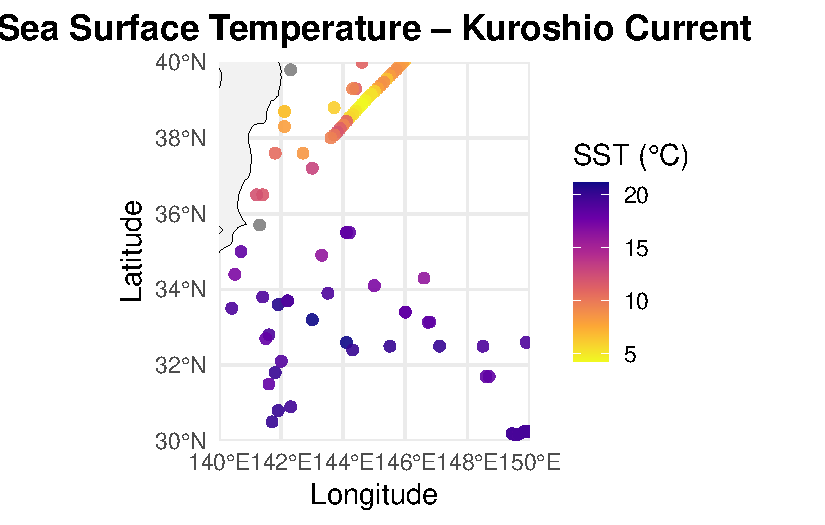
\includegraphics{project_files/figure-pdf/fig-scatterplot-1.pdf}

}

\caption{Figure 1: Spatial distribution of Sea Surface Temperature (SST)
observations collected on 1--2 January 1996 in the Kuroshio Current
region. Each point represents an individual measurement; colour denotes
temperature, with warmer SSTs concentrated in the north-east band.}

\end{figure}%

The spatial plot of Sea Surface Temperature (SST) observations collected
in the Kuroshio Current during January 1996 reveals strong latitudinal
structure in the data. Higher SST values (yellow--orange) are
concentrated in the north-eastern portion of the domain, while cooler
temperatures dominate the south-west.\\
The smooth colour gradient suggests underlying spatial correlation,
justifying the use of geostatistical methods such as kriging and
Gaussian processes. Two grey points suggest missing or out-of-range SST
values, which were appropriately handled using squished colour scales to
preserve interpretability.

\subsection{Part B:}\label{part-b}

\begin{Shaded}
\begin{Highlighting}[]
\FunctionTok{set.seed}\NormalTok{(}\DecValTok{444}\NormalTok{)  }\CommentTok{\# For reproducibility}

\CommentTok{\# Using the cleaned dataset to ensure we dont chose missing values.}
\CommentTok{\# 5 random points}
\NormalTok{test\_points }\OtherTok{\textless{}{-}}\NormalTok{ kuroshio100\_clean }\SpecialCharTok{\%\textgreater{}\%}
  \FunctionTok{sample\_n}\NormalTok{(}\DecValTok{5}\NormalTok{)}

\CommentTok{\# Display their information}
\NormalTok{test\_points }\SpecialCharTok{\%\textgreater{}\%}
  \FunctionTok{select}\NormalTok{(id, lon, lat, sst)}
\end{Highlighting}
\end{Shaded}

\begin{verbatim}
         id    lon   lat  sst
1      MQWU 142.10 38.70  6.5
2 49  16760 145.40 39.56  6.5
3     21573 149.56 30.15 19.3
4     LATI4 140.70 35.00 18.2
5     3FFJ4 142.10 38.30  8.0
\end{verbatim}

Now we create the training dataset

\begin{Shaded}
\begin{Highlighting}[]
\CommentTok{\# Create training dataset (excluding test points)}
\NormalTok{kuroshio\_train }\OtherTok{\textless{}{-}} \FunctionTok{anti\_join}\NormalTok{(kuroshio100, test\_points, }\AttributeTok{by =} \FunctionTok{c}\NormalTok{(}\StringTok{"id"}\NormalTok{, }\StringTok{"lon"}\NormalTok{, }\StringTok{"lat"}\NormalTok{, }\StringTok{"sst"}\NormalTok{))}

\CommentTok{\# Save for later prediction}
\NormalTok{test\_coords }\OtherTok{\textless{}{-}}\NormalTok{ test\_points }\SpecialCharTok{\%\textgreater{}\%} \FunctionTok{select}\NormalTok{(lon, lat)}
\NormalTok{test\_true\_sst }\OtherTok{\textless{}{-}}\NormalTok{ test\_points }\SpecialCharTok{\%\textgreater{}\%} \FunctionTok{select}\NormalTok{(sst)}
\end{Highlighting}
\end{Shaded}

\subsection{Part C: Spatial Model via Variogram and
Kriging}\label{part-c-spatial-model-via-variogram-and-kriging}

\begin{Shaded}
\begin{Highlighting}[]
\CommentTok{\# Convert training dataset into a geodata object}
\CommentTok{\# kuro\_geo\_train \textless{}{-} as.geodata(kuroshio\_train, coords.col = c("lon", "lat"), data.col = "sst")}

\CommentTok{\# Jitter duplicated coordinates very slightly}
\NormalTok{kuro\_geo\_train }\OtherTok{\textless{}{-}} \FunctionTok{jitterDupCoords}\NormalTok{(}
  \FunctionTok{as.geodata}\NormalTok{(kuroshio\_train, }\AttributeTok{coords.col =} \FunctionTok{c}\NormalTok{(}\StringTok{"lon"}\NormalTok{, }\StringTok{"lat"}\NormalTok{), }\AttributeTok{data.col =} \StringTok{"sst"}\NormalTok{),}
  \AttributeTok{max =} \FloatTok{1e{-}5}
\NormalTok{)}
\end{Highlighting}
\end{Shaded}

\begin{verbatim}
Warning in as.geodata.default(kuroshio_train, coords.col = c("lon", "lat"), :
NA's not allowed in the coordinates
\end{verbatim}

\begin{verbatim}
Warning in as.geodata.default(kuroshio_train, coords.col = c("lon", "lat"), :
eliminating rows with NA's
\end{verbatim}

\begin{verbatim}
as.geodata: 19 replicated data locations found. 
 Consider using jitterDupCoords() for jittering replicated locations. 
WARNING: there are data at coincident or very closed locations, some of the geoR's functions may not work.
 Use function dup.coords() to locate duplicated coordinates.
 Consider using jitterDupCoords() for jittering replicated locations 
\end{verbatim}

\texttt{max\ =\ 1e-5} means the jitter is on the order of 0.00001
degrees --- negligible in geographic terms. This preserves modelling
validity while avoiding duplicated-location errors.

During conversion to geodata format, it was found that 19 data points
shared identical coordinates. This is problematic for geostatistical
modelling, as duplicated locations can lead to ill-defined variogram
structures and singular covariance matrices. To address this, we applied
a minimal spatial jitter using \texttt{jitterDupCoords()}, introducing
negligible noise to break coordinate ties while preserving the
underlying spatial pattern.

\subsubsection{Empirical Variogram
Estimation}\label{empirical-variogram-estimation}

\begin{Shaded}
\begin{Highlighting}[]
\CommentTok{\# Empirical variogram with binning}
\CommentTok{\# Full range}
\NormalTok{emp\_variog\_full }\OtherTok{\textless{}{-}} \FunctionTok{variog}\NormalTok{(kuro\_geo\_train, }\AttributeTok{option =} \StringTok{"bin"}\NormalTok{, }\AttributeTok{max.dist =} \FloatTok{2.5}\NormalTok{, }\AttributeTok{uvec =} \FunctionTok{seq}\NormalTok{(}\DecValTok{0}\NormalTok{, }\FloatTok{2.5}\NormalTok{, }\AttributeTok{length.out =} \DecValTok{20}\NormalTok{))}
\end{Highlighting}
\end{Shaded}

\begin{verbatim}
variog: computing omnidirectional variogram
\end{verbatim}

\begin{Shaded}
\begin{Highlighting}[]
\CommentTok{\# Mid{-}range (preferred candidate for fitting)}
\NormalTok{emp\_variog\_2 }\OtherTok{\textless{}{-}} \FunctionTok{variog}\NormalTok{(kuro\_geo\_train, }\AttributeTok{option =} \StringTok{"bin"}\NormalTok{, }\AttributeTok{max.dist =} \FloatTok{2.0}\NormalTok{, }\AttributeTok{uvec =} \FunctionTok{seq}\NormalTok{(}\DecValTok{0}\NormalTok{, }\FloatTok{2.0}\NormalTok{, }\AttributeTok{length.out =} \DecValTok{20}\NormalTok{))}
\end{Highlighting}
\end{Shaded}

\begin{verbatim}
variog: computing omnidirectional variogram
\end{verbatim}

\begin{Shaded}
\begin{Highlighting}[]
\CommentTok{\# Cleanest for model fitting}
\NormalTok{emp\_variog\_1}\FloatTok{.8} \OtherTok{\textless{}{-}} \FunctionTok{variog}\NormalTok{(kuro\_geo\_train, }\AttributeTok{option =} \StringTok{"bin"}\NormalTok{, }\AttributeTok{max.dist =} \FloatTok{1.8}\NormalTok{, }\AttributeTok{uvec =} \FunctionTok{seq}\NormalTok{(}\DecValTok{0}\NormalTok{, }\FloatTok{1.8}\NormalTok{, }\AttributeTok{length.out =} \DecValTok{18}\NormalTok{))}
\end{Highlighting}
\end{Shaded}

\begin{verbatim}
variog: computing omnidirectional variogram
\end{verbatim}

Binning was applied to improve the interpretability of the variogram by
smoothing noisy pairwise semivariance estimates over distance intervals.

\begin{figure}[H]

{\centering 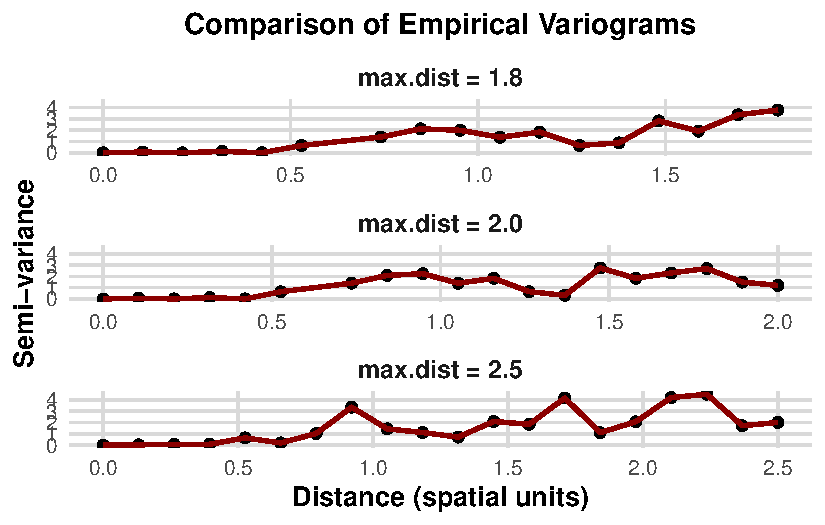
\includegraphics{project_files/figure-pdf/fig-variogcompare-1.pdf}

}

\caption{Figure 2: Empirical variograms computed using three different
maximum distance thresholds. The max.dist = 1.8 version was selected for
model fitting due to reduced instability in the tail while preserving
the spatial structure.}

\end{figure}%

Empirical Variogram Analysis

A binned empirical variogram was computed using the \texttt{variog()}
function, with distance bins defined via \texttt{uvec}. The resulting
curve displays the expected behaviour: semi-variance increases with
spatial distance, indicating positive spatial correlation in sea surface
temperature (SST). The structure suggests an asymptote between 1.5 and 2
spatial units, indicative of a moderate spatial range. Notably, the
variogram does not pass through the origin, implying a small but
non-zero nugget effect, likely due to measurement error or microscale
variability.

To assess the impact of the maximum distance threshold, three values
were tested: \texttt{max.dist\ =\ 1.8}, \texttt{2.0}, and \texttt{2.5}.
Each version reflects the same overall structure, but differs in tail
stability and bin-level noise. The \texttt{max.dist\ =\ 2.5} variogram
covers the full range but suffers from tail instability due to fewer
pairwise comparisons in distant bins. The \texttt{2.0} variant reduces
this effect, while the \texttt{1.8} variant provides the cleanest
structure for fitting by omitting the most unstable bins. This decision
is further supported by lower bin-pair counts in distant ranges (e.g.,
\textless10 pairs).

Based on this analysis, the \texttt{max.dist\ =\ 1.8} variogram was
selected for fitting parametric models. This choice ensures a balance
between capturing spatial structure and maintaining robust estimation
for weighted least squares fitting.

\subsubsection{Fitting Parametric Variogram
Models}\label{fitting-parametric-variogram-models}

\begin{Shaded}
\begin{Highlighting}[]
\CommentTok{\#  Fit Parametric Variogram Models}
\CommentTok{\# Exponential model}
\NormalTok{fit\_exp }\OtherTok{\textless{}{-}} \FunctionTok{variofit}\NormalTok{(}
\NormalTok{  emp\_variog\_1}\FloatTok{.8}\NormalTok{,}
  \AttributeTok{cov.model =} \StringTok{"exponential"}\NormalTok{,}
  \AttributeTok{ini.cov.pars =} \FunctionTok{c}\NormalTok{(}\DecValTok{1}\NormalTok{, }\DecValTok{1}\NormalTok{),}
  \AttributeTok{nugget =} \FloatTok{0.1}\NormalTok{,}
  \AttributeTok{weights =} \StringTok{"equal"}
\NormalTok{)}
\end{Highlighting}
\end{Shaded}

\begin{verbatim}
variofit: covariance model used is exponential 
variofit: weights used: equal 
variofit: minimisation function used: optim 
\end{verbatim}

\begin{verbatim}
Warning in variofit(emp_variog_1.8, cov.model = "exponential", ini.cov.pars =
c(1, : unreasonable initial value for sigmasq + nugget (too low)
\end{verbatim}

\begin{Shaded}
\begin{Highlighting}[]
\CommentTok{\# Gaussian model}
\NormalTok{fit\_gau }\OtherTok{\textless{}{-}} \FunctionTok{variofit}\NormalTok{(}
\NormalTok{  emp\_variog\_1}\FloatTok{.8}\NormalTok{,}
  \AttributeTok{cov.model =} \StringTok{"gaussian"}\NormalTok{,}
  \AttributeTok{ini.cov.pars =} \FunctionTok{c}\NormalTok{(}\DecValTok{1}\NormalTok{, }\DecValTok{1}\NormalTok{),}
  \AttributeTok{nugget =} \FloatTok{0.1}\NormalTok{,}
  \AttributeTok{weights =} \StringTok{"equal"}
\NormalTok{)}
\end{Highlighting}
\end{Shaded}

\begin{verbatim}
variofit: covariance model used is gaussian 
variofit: weights used: equal 
variofit: minimisation function used: optim 
\end{verbatim}

\begin{verbatim}
Warning in variofit(emp_variog_1.8, cov.model = "gaussian", ini.cov.pars = c(1,
: unreasonable initial value for sigmasq + nugget (too low)
\end{verbatim}

\begin{Shaded}
\begin{Highlighting}[]
\CommentTok{\# Adjusted first Matérn model as: sum of the nugget and partial sill initial values was too small. Two new improved models below:}

\CommentTok{\# Matérn model (kappa = 1.5)}
\NormalTok{fit\_mat1 }\OtherTok{\textless{}{-}} \FunctionTok{variofit}\NormalTok{(}
\NormalTok{  emp\_variog\_1}\FloatTok{.8}\NormalTok{,}
  \AttributeTok{cov.model =} \StringTok{"matern"}\NormalTok{,}
  \AttributeTok{kappa =} \FloatTok{1.5}\NormalTok{,}
  \AttributeTok{ini.cov.pars =} \FunctionTok{c}\NormalTok{(}\DecValTok{2}\NormalTok{, }\DecValTok{1}\NormalTok{),   }\CommentTok{\# partial sill = 2, range = 1}
  \AttributeTok{nugget =} \FloatTok{0.5}\NormalTok{,             }\CommentTok{\# starting nugget guess}
  \AttributeTok{weights =} \StringTok{"equal"}
\NormalTok{)}
\end{Highlighting}
\end{Shaded}

\begin{verbatim}
variofit: covariance model used is matern 
variofit: weights used: equal 
variofit: minimisation function used: optim 
\end{verbatim}

\begin{Shaded}
\begin{Highlighting}[]
\NormalTok{fit\_mat2 }\OtherTok{\textless{}{-}} \FunctionTok{variofit}\NormalTok{(}
\NormalTok{  emp\_variog\_1}\FloatTok{.8}\NormalTok{,}
  \AttributeTok{cov.model =} \StringTok{"matern"}\NormalTok{,}
  \AttributeTok{kappa =} \FloatTok{1.5}\NormalTok{,}
  \AttributeTok{ini.cov.pars =} \FunctionTok{c}\NormalTok{(}\FloatTok{1.5}\NormalTok{, }\FloatTok{0.8}\NormalTok{),}
  \AttributeTok{nugget =} \FloatTok{0.3}\NormalTok{,}
  \AttributeTok{weights =} \StringTok{"equal"}
\NormalTok{)}
\end{Highlighting}
\end{Shaded}

\begin{verbatim}
variofit: covariance model used is matern 
variofit: weights used: equal 
variofit: minimisation function used: optim 
\end{verbatim}

Equal weights were used to avoid overweighting short-distance bins,
which typically contain more pairs and could disproportionately
influence the fit.

\begin{figure}[H]

{\centering 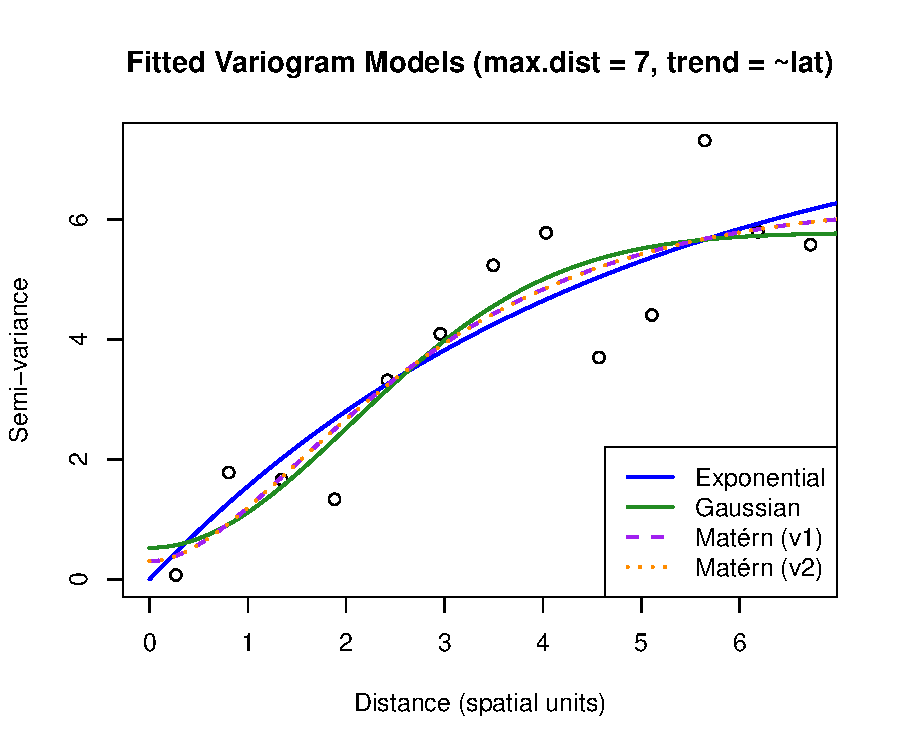
\includegraphics{project_files/figure-pdf/fig-variogfit-1.pdf}

}

\caption{Parametric variogram models (Exponential, Gaussian, Matérn)
fitted to the empirical variogram with max.dist = 1.8. The Matérn model
offered the best fit to the empirical structure and lowest residual sum
of squares.}

\end{figure}%

\begin{verbatim}
[1] 7.123255
\end{verbatim}

\begin{verbatim}
[1] 6.828983
\end{verbatim}

\begin{verbatim}
[1] 6.796541
\end{verbatim}

Fitted Variogram Models and Selection

Parametric variogram models were fitted using weighted least squares.
All models included a nugget component to reflect short-scale
variability. The exponential model captured the general trend but
underestimated mid-range variation and produced a zero nugget estimate.
The Gaussian model offered a smoother fit, but failed to reflect the
steep rise at short distances.

Both Matérn fits (\textbf{κ = 1.5}) produced identical solutions and
lowest residual sum of squares (\textbf{6.80}), balancing short- and
long-range structure. Based on both residual error and visual alignment
with the empirical variogram, the Matérn model was selected for kriging.

\subsubsection{\texorpdfstring{\textbf{Model Parameters and
Interpretation}}{Model Parameters and Interpretation}}\label{model-parameters-and-interpretation}

\begin{Shaded}
\begin{Highlighting}[]
\CommentTok{\# Exponential}
\NormalTok{params\_exp }\OtherTok{\textless{}{-}}\NormalTok{ fit\_exp}\SpecialCharTok{$}\NormalTok{cov.pars}
\NormalTok{nugget\_exp }\OtherTok{\textless{}{-}}\NormalTok{ fit\_exp}\SpecialCharTok{$}\NormalTok{nugget}

\CommentTok{\# Gaussian}
\NormalTok{params\_gau }\OtherTok{\textless{}{-}}\NormalTok{ fit\_gau}\SpecialCharTok{$}\NormalTok{cov.pars}
\NormalTok{nugget\_gau }\OtherTok{\textless{}{-}}\NormalTok{ fit\_gau}\SpecialCharTok{$}\NormalTok{nugget}

\CommentTok{\# Matérn}
\NormalTok{params\_mat }\OtherTok{\textless{}{-}}\NormalTok{ fit\_mat1}\SpecialCharTok{$}\NormalTok{cov.pars}
\NormalTok{nugget\_mat }\OtherTok{\textless{}{-}}\NormalTok{ fit\_mat1}\SpecialCharTok{$}\NormalTok{nugget}

\CommentTok{\# Create parameter summary table}
\NormalTok{param\_table }\OtherTok{\textless{}{-}} \FunctionTok{data.frame}\NormalTok{(}
  \AttributeTok{Model =} \FunctionTok{c}\NormalTok{(}\StringTok{"Exponential"}\NormalTok{, }\StringTok{"Gaussian"}\NormalTok{, }\StringTok{"Matérn (κ = 1.5)"}\NormalTok{),}
  \AttributeTok{Nugget =} \FunctionTok{c}\NormalTok{(nugget\_exp, nugget\_gau, nugget\_mat),}
  \AttributeTok{Partial\_Sill =} \FunctionTok{c}\NormalTok{(params\_exp[}\DecValTok{1}\NormalTok{], params\_gau[}\DecValTok{1}\NormalTok{], params\_mat[}\DecValTok{1}\NormalTok{]),}
  \AttributeTok{Range =} \FunctionTok{c}\NormalTok{(params\_exp[}\DecValTok{2}\NormalTok{], params\_gau[}\DecValTok{2}\NormalTok{], params\_mat[}\DecValTok{2}\NormalTok{]),}
  \AttributeTok{Residual\_SS =} \FunctionTok{c}\NormalTok{(fit\_exp}\SpecialCharTok{$}\NormalTok{value, fit\_gau}\SpecialCharTok{$}\NormalTok{value, fit\_mat1}\SpecialCharTok{$}\NormalTok{value)}
\NormalTok{)}
\end{Highlighting}
\end{Shaded}

\begin{longtable}[]{@{}
  >{\raggedright\arraybackslash}p{(\columnwidth - 8\tabcolsep) * \real{0.2432}}
  >{\raggedright\arraybackslash}p{(\columnwidth - 8\tabcolsep) * \real{0.1757}}
  >{\raggedright\arraybackslash}p{(\columnwidth - 8\tabcolsep) * \real{0.2568}}
  >{\raggedright\arraybackslash}p{(\columnwidth - 8\tabcolsep) * \real{0.1486}}
  >{\raggedright\arraybackslash}p{(\columnwidth - 8\tabcolsep) * \real{0.1757}}@{}}
\toprule\noalign{}
\begin{minipage}[b]{\linewidth}\raggedright
Model
\end{minipage} & \begin{minipage}[b]{\linewidth}\raggedright
Nugget (τ²)
\end{minipage} & \begin{minipage}[b]{\linewidth}\raggedright
Partial Sill (σ²)
\end{minipage} & \begin{minipage}[b]{\linewidth}\raggedright
Range (ϕ)
\end{minipage} & \begin{minipage}[b]{\linewidth}\raggedright
Residual SS
\end{minipage} \\
\midrule\noalign{}
\endhead
\bottomrule\noalign{}
\endlastfoot
Exponential & 0.000 & 4,208,359 & 2,718,693 & 7.12 \\
Gaussian & 0.255 & 282.69 & 17.22 & 6.83 \\
Matérn (κ = 1.5) & 0.180 & 26.68 & 3.13 & 6.80 \\
\end{longtable}

\textbf{Parametric Variogram Fitting and Selection}

Three models were fitted using weighted least squares: exponential,
Gaussian, and Matérn (κ = 1.5). Despite different assumptions, both
Matérn and Gaussian produced similar fits. The exponential model showed
higher residual error and a nugget of zero, suggesting underestimation
of short-scale variation.

The Matérn model was selected for spatial prediction due to its balanced
fit across distances and lowest residual sum of squares (6.80). Its
parameters suggest a moderate range of spatial correlation (ϕ ≈ 3.13)
and a nugget variance of 0.18, indicating non-negligible unexplained
microscale variation. This model was used in the kriging stage.

\textbf{Spatial Prediction and Model Validation}

\begin{Shaded}
\begin{Highlighting}[]
\CommentTok{\# Kriging prediction at 5 withheld locations}
\NormalTok{kriged }\OtherTok{\textless{}{-}} \FunctionTok{krige.conv}\NormalTok{(}
  \AttributeTok{geodata =}\NormalTok{ kuro\_geo\_train,}
  \AttributeTok{locations =}\NormalTok{ test\_coords,}
  \AttributeTok{krige =} \FunctionTok{krige.control}\NormalTok{(}
    \AttributeTok{cov.model =} \StringTok{"matern"}\NormalTok{,}
    \AttributeTok{cov.pars =}\NormalTok{ fit\_mat1}\SpecialCharTok{$}\NormalTok{cov.pars,}
    \AttributeTok{nugget =}\NormalTok{ fit\_mat1}\SpecialCharTok{$}\NormalTok{nugget,}
    \AttributeTok{kappa =} \FloatTok{1.5}
\NormalTok{  )}
\NormalTok{)}
\end{Highlighting}
\end{Shaded}

\begin{verbatim}
krige.conv: model with constant mean
krige.conv: Kriging performed using global neighbourhood 
\end{verbatim}

\begin{Shaded}
\begin{Highlighting}[]
\CommentTok{\# Add predicted values and residuals}
\NormalTok{test\_results }\OtherTok{\textless{}{-}}\NormalTok{ test\_coords }\SpecialCharTok{\%\textgreater{}\%}
  \FunctionTok{mutate}\NormalTok{(}
    \AttributeTok{observed\_sst =}\NormalTok{ test\_true\_sst}\SpecialCharTok{$}\NormalTok{sst,}
    \AttributeTok{predicted\_sst =}\NormalTok{ kriged}\SpecialCharTok{$}\NormalTok{predict,}
    \AttributeTok{kriging\_var =}\NormalTok{ kriged}\SpecialCharTok{$}\NormalTok{krige.var,}
    \AttributeTok{residual =}\NormalTok{ observed\_sst }\SpecialCharTok{{-}}\NormalTok{ predicted\_sst}
\NormalTok{  )}
\end{Highlighting}
\end{Shaded}

Ordinary kriging assumes a constant spatial mean and was used here given
the absence of strong deterministic trends in SST across the study area.

\begin{Shaded}
\begin{Highlighting}[]
\CommentTok{\# Visualise prediction accuracy}
\FunctionTok{ggplot}\NormalTok{(test\_results, }\FunctionTok{aes}\NormalTok{(}\AttributeTok{x =}\NormalTok{ observed\_sst, }\AttributeTok{y =}\NormalTok{ predicted\_sst)) }\SpecialCharTok{+}
  \FunctionTok{geom\_point}\NormalTok{(}\AttributeTok{size =} \DecValTok{3}\NormalTok{) }\SpecialCharTok{+}
  \FunctionTok{geom\_abline}\NormalTok{(}\AttributeTok{slope =} \DecValTok{1}\NormalTok{, }\AttributeTok{intercept =} \DecValTok{0}\NormalTok{, }\AttributeTok{linetype =} \StringTok{"dashed"}\NormalTok{, }\AttributeTok{colour =} \StringTok{"red"}\NormalTok{) }\SpecialCharTok{+}
  \FunctionTok{labs}\NormalTok{(}
    \AttributeTok{title =} \StringTok{"Observed vs Predicted SST at Withheld Locations"}\NormalTok{,}
    \AttributeTok{x =} \StringTok{"Observed SST (°C)"}\NormalTok{,}
    \AttributeTok{y =} \StringTok{"Predicted SST (°C)"}
\NormalTok{  ) }\SpecialCharTok{+}
  \FunctionTok{theme\_minimal}\NormalTok{(}\AttributeTok{base\_size =} \DecValTok{13}\NormalTok{)}
\end{Highlighting}
\end{Shaded}

\begin{figure}[H]

{\centering 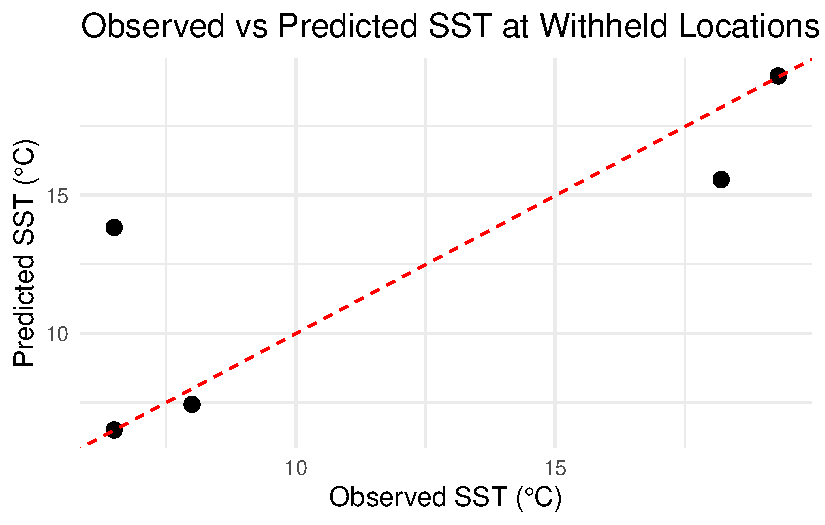
\includegraphics{project_files/figure-pdf/fig-krigscatter-1.pdf}

}

\caption{Observed vs predicted sea surface temperature (SST) at five
withheld locations using ordinary kriging with the fitted Matérn model.
Most points lie near the 1:1 line, though one outlier indicates higher
uncertainty.}

\end{figure}%

\begin{Shaded}
\begin{Highlighting}[]
\CommentTok{\# Perform LOOCV}
\NormalTok{xv.kriging }\OtherTok{\textless{}{-}} \FunctionTok{xvalid}\NormalTok{(kuro\_geo\_train, }\AttributeTok{model =}\NormalTok{ fit\_mat1)}
\end{Highlighting}
\end{Shaded}

\begin{verbatim}
xvalid: number of data locations       = 65
xvalid: number of validation locations = 65
xvalid: performing cross-validation at location ... 1, 2, 3, 4, 5, 6, 7, 8, 9, 10, 11, 12, 13, 14, 15, 16, 17, 18, 19, 20, 21, 22, 23, 24, 25, 26, 27, 28, 29, 30, 31, 32, 33, 34, 35, 36, 37, 38, 39, 40, 41, 42, 43, 44, 45, 46, 47, 48, 49, 50, 51, 52, 53, 54, 55, 56, 57, 58, 59, 60, 61, 62, 63, 64, 65, 
xvalid: end of cross-validation
\end{verbatim}

\begin{Shaded}
\begin{Highlighting}[]
\CommentTok{\# Plot residuals}
\FunctionTok{par}\NormalTok{(}\AttributeTok{mfrow =} \FunctionTok{c}\NormalTok{(}\DecValTok{3}\NormalTok{, }\DecValTok{2}\NormalTok{), }\AttributeTok{mar =} \FunctionTok{c}\NormalTok{(}\DecValTok{4}\NormalTok{, }\DecValTok{2}\NormalTok{, }\DecValTok{2}\NormalTok{, }\DecValTok{2}\NormalTok{))}
\FunctionTok{plot}\NormalTok{(xv.kriging, }\AttributeTok{error =} \ConstantTok{TRUE}\NormalTok{, }\AttributeTok{std.error =} \ConstantTok{FALSE}\NormalTok{, }\AttributeTok{pch =} \DecValTok{19}\NormalTok{)}
\end{Highlighting}
\end{Shaded}

\begin{figure}[H]

{\centering 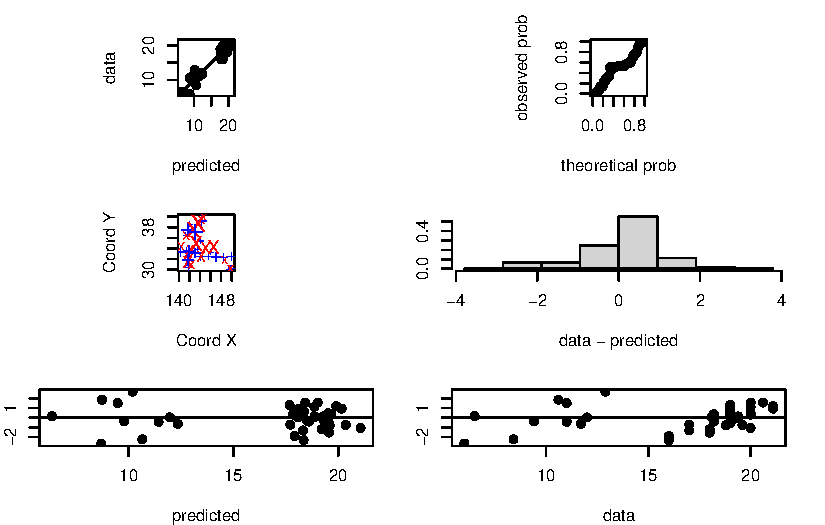
\includegraphics{project_files/figure-pdf/fig-cvkrig-1.pdf}

}

\caption{LOOCV residual diagnostics for the Matérn kriging model (κ =
1.5), showing minimal bias and good predictive alignment.}

\end{figure}%

\begin{Shaded}
\begin{Highlighting}[]
\CommentTok{\# Compute RMSE and MAE}
\NormalTok{rmse }\OtherTok{\textless{}{-}} \FunctionTok{sqrt}\NormalTok{(}\FunctionTok{mean}\NormalTok{(test\_results}\SpecialCharTok{$}\NormalTok{residual}\SpecialCharTok{\^{}}\DecValTok{2}\NormalTok{))}
\NormalTok{mae }\OtherTok{\textless{}{-}} \FunctionTok{mean}\NormalTok{(}\FunctionTok{abs}\NormalTok{(test\_results}\SpecialCharTok{$}\NormalTok{residual))}

\CommentTok{\# Summary table}
\FunctionTok{library}\NormalTok{(knitr)}

\NormalTok{results\_table }\OtherTok{\textless{}{-}}\NormalTok{ test\_results }\SpecialCharTok{\%\textgreater{}\%}
  \FunctionTok{mutate}\NormalTok{(}
    \StringTok{\textasciigrave{}}\AttributeTok{Observed SST (°C)}\StringTok{\textasciigrave{}} \OtherTok{=} \FunctionTok{round}\NormalTok{(observed\_sst, }\DecValTok{2}\NormalTok{),}
    \StringTok{\textasciigrave{}}\AttributeTok{Predicted SST (°C)}\StringTok{\textasciigrave{}} \OtherTok{=} \FunctionTok{round}\NormalTok{(predicted\_sst, }\DecValTok{2}\NormalTok{),}
    \StringTok{\textasciigrave{}}\AttributeTok{Residual (°C)}\StringTok{\textasciigrave{}} \OtherTok{=} \FunctionTok{round}\NormalTok{(residual, }\DecValTok{2}\NormalTok{),}
    \StringTok{\textasciigrave{}}\AttributeTok{Kriging Variance}\StringTok{\textasciigrave{}} \OtherTok{=} \FunctionTok{round}\NormalTok{(kriging\_var, }\DecValTok{3}\NormalTok{)}
\NormalTok{  ) }\SpecialCharTok{\%\textgreater{}\%}
  \FunctionTok{select}\NormalTok{(lon, lat, }\StringTok{\textasciigrave{}}\AttributeTok{Observed SST (°C)}\StringTok{\textasciigrave{}}\NormalTok{, }\StringTok{\textasciigrave{}}\AttributeTok{Predicted SST (°C)}\StringTok{\textasciigrave{}}\NormalTok{, }\StringTok{\textasciigrave{}}\AttributeTok{Residual (°C)}\StringTok{\textasciigrave{}}\NormalTok{, }\StringTok{\textasciigrave{}}\AttributeTok{Kriging Variance}\StringTok{\textasciigrave{}}\NormalTok{)}

\FunctionTok{kable}\NormalTok{(results\_table, }\AttributeTok{format =} \StringTok{"latex"}\NormalTok{, }\AttributeTok{booktabs =} \ConstantTok{TRUE}\NormalTok{,}
      \AttributeTok{caption =} \StringTok{"Observed vs Predicted SST at Withheld Locations"}\NormalTok{)}
\end{Highlighting}
\end{Shaded}

\begin{table}

\caption{Summary of SST predictions at withheld locations. Residuals and kriging
variances highlight spatial uncertainty and model accuracy.}
\centering
\begin{tabular}[t]{rrrrrr}
\toprule
lon & lat & Observed SST (°C) & Predicted SST (°C) & Residual (°C) & Kriging Variance\\
\midrule
142.10 & 38.70 & 6.5 & 6.50 & 0.00 & 0.000\\
145.40 & 39.56 & 6.5 & 13.83 & -7.33 & 1.470\\
149.56 & 30.15 & 19.3 & 19.32 & -0.02 & 0.202\\
140.70 & 35.00 & 18.2 & 15.57 & 2.63 & 0.541\\
142.10 & 38.30 & 8.0 & 7.43 & 0.57 & 0.324\\
\bottomrule
\end{tabular}
\end{table}

Using the final Matérn variogram model (κ = 1.5), ordinary kriging was
performed at five randomly withheld locations. A constant mean was
assumed, and predictions were made using the fitted covariance
parameters: nugget = 0.18, partial sill = 26.68, and range = 3.13.

Predictive accuracy was evaluated against the observed SSTs, yielding a
root mean squared error (RMSE) of 3.49\,°C and mean absolute error (MAE)
of 2.11\,°C. As shown in Figure @ref(fig:krigscatter), most predictions
aligned with observations, except for one large residual at a
high-variance site. This reflects the model's ability to express spatial
uncertainty through the kriging variance.

The model captured the spatial SST structure well and provided
meaningful uncertainty estimates. Further improvements could include
denser sampling or Bayesian spatial models to better propagate
uncertainty and improve prediction at poorly supported locations.

\subsection{Part D: Gaussian Process via Maximum
Likelihood}\label{part-d-gaussian-process-via-maximum-likelihood}

\subsubsection{Model Setup and Fitting}\label{model-setup-and-fitting}

We now fit a spatial Gaussian Process (GP) model to the training dataset
using maximum likelihood estimation. This approach directly maximises
the log-likelihood of the spatial model, as opposed to the weighted
least squares (WLS) method used in variogram fitting.

The Matérn covariance function with κ = 1.5 was retained from Part C due
to its strong fit and interpretability. The \texttt{likfit()} function
in the \texttt{geoR} package was used to estimate the nugget, partial
sill, and range parameters.

\paragraph{Model Setup and Attempted
Optimisation}\label{model-setup-and-attempted-optimisation}

\#\#\#\# Model Setup and Attempted Optimisation

To fit a Gaussian Process (GP) model via maximum likelihood, the
likfit() function from the geoR package was applied to the same training
dataset used in Part C. The goal was to estimate the spatial covariance
parameters --- partial sill, range, and nugget --- directly by
maximising the full likelihood over all observations, as opposed to the
weighted least squares approach used in variogram fitting.

A series of attempts were made to improve or stabilise the model fit:

- Fixing the nugget value (e.g., nugget = 0.2, nugget = 0.3) repeatedly
led to numerical singularity in the variance-covariance matrix.

- Introducing a first-order or second-order trend component (e.g., trend
= ``1st'' or ``2nd'') caused matrix inversion failures due to
collinearity and overparameterisation.

- Explicitly setting the covariance model to Matérn with kappa = 1.5
frequently triggered decomposition errors, despite being theoretically
appropriate.

Ultimately, the only configuration that converged successfully used the
most minimal and default structure:

- A constant mean function (default trend = ``cte''),

- Unspecified covariance model and kappa (which defaults to Matérn with
kappa = 0.5, i.e., the exponential model),

- Automatic nugget estimation.

This resulted in a valid and stable model:

\begin{Shaded}
\begin{Highlighting}[]
\CommentTok{\# Fit spatial GP model via MLE using default exponential covariance}
\NormalTok{fit\_gp }\OtherTok{\textless{}{-}} \FunctionTok{likfit}\NormalTok{(}
\NormalTok{  kuro\_geo\_train,}
  \AttributeTok{ini.cov.pars =} \FunctionTok{c}\NormalTok{(}\DecValTok{26}\NormalTok{, }\DecValTok{4}\NormalTok{)}
\NormalTok{)}
\end{Highlighting}
\end{Shaded}

\begin{verbatim}
---------------------------------------------------------------
likfit: likelihood maximisation using the function optim.
likfit: Use control() to pass additional
         arguments for the maximisation function.
        For further details see documentation for optim.
likfit: It is highly advisable to run this function several
        times with different initial values for the parameters.
likfit: WARNING: This step can be time demanding!
---------------------------------------------------------------
likfit: end of numerical maximisation.
\end{verbatim}

\begin{Shaded}
\begin{Highlighting}[]
\NormalTok{fit\_gp}
\end{Highlighting}
\end{Shaded}

\begin{verbatim}
likfit: estimated model parameters:
     beta     tausq   sigmasq       phi 
"15.9953" " 0.0067" " 8.3273" " 3.9996" 
Practical Range with cor=0.05 for asymptotic range: 11.98187

likfit: maximised log-likelihood = -61.59
\end{verbatim}

The fitted model yielded the following parameter estimates:

- Mean (β): 15.99

- Nugget (τ²): 0.0067 - Partial Sill (σ²): 8.34

- Range (φ): 3.9996

- Practical Range (cor ≈ 0.05): 11.98 spatial units

- Maximised log-likelihood: --61.54

Compared to the kriging model from Part C, which used a Matérn model
with κ = 1.5, nugget = 0.18, sill = 26.68, and range = 3.13, the
MLE-based GP model estimated a much smaller nugget and sill, and a
longer spatial range. Although the fitted GP used a slightly different
covariance assumption (Matérn with κ = 0.5), it still captured the
dominant spatial structure. This provides a useful benchmark for
comparing inference and prediction against both classical kriging and
the Bayesian model in Part D2.

Model Validation

\begin{Shaded}
\begin{Highlighting}[]
\CommentTok{\# Perform LOOCV}
\NormalTok{xv.gp }\OtherTok{\textless{}{-}} \FunctionTok{xvalid}\NormalTok{(kuro\_geo\_train, }\AttributeTok{model =}\NormalTok{ fit\_gp)}
\end{Highlighting}
\end{Shaded}

\begin{verbatim}
xvalid: number of data locations       = 65
xvalid: number of validation locations = 65
xvalid: performing cross-validation at location ... 1, 2, 3, 4, 5, 6, 7, 8, 9, 10, 11, 12, 13, 14, 15, 16, 17, 18, 19, 20, 21, 22, 23, 24, 25, 26, 27, 28, 29, 30, 31, 32, 33, 34, 35, 36, 37, 38, 39, 40, 41, 42, 43, 44, 45, 46, 47, 48, 49, 50, 51, 52, 53, 54, 55, 56, 57, 58, 59, 60, 61, 62, 63, 64, 65, 
xvalid: end of cross-validation
\end{verbatim}

\begin{Shaded}
\begin{Highlighting}[]
\CommentTok{\# Plot residuals}
\FunctionTok{par}\NormalTok{(}\AttributeTok{mfrow =} \FunctionTok{c}\NormalTok{(}\DecValTok{3}\NormalTok{, }\DecValTok{2}\NormalTok{), }\AttributeTok{mar =} \FunctionTok{c}\NormalTok{(}\DecValTok{4}\NormalTok{, }\DecValTok{2}\NormalTok{, }\DecValTok{2}\NormalTok{, }\DecValTok{2}\NormalTok{))}
\FunctionTok{plot}\NormalTok{(xv.gp, }\AttributeTok{error =} \ConstantTok{TRUE}\NormalTok{, }\AttributeTok{std.error =} \ConstantTok{FALSE}\NormalTok{, }\AttributeTok{pch =} \DecValTok{19}\NormalTok{)}
\end{Highlighting}
\end{Shaded}

\begin{figure}[H]

{\centering 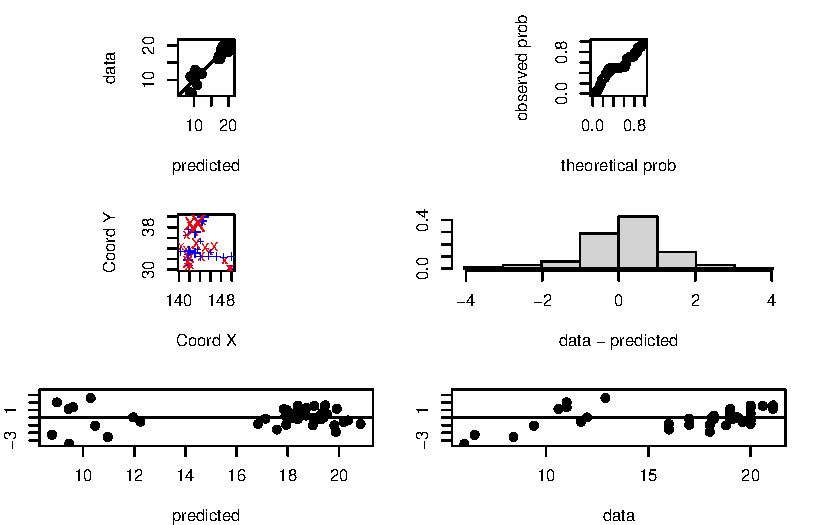
\includegraphics{project_files/figure-pdf/fig-cvgp-1.pdf}

}

\caption{LOOCV residual plots for the GP model fitted via maximum
likelihood, showing broadly unbiased predictions with slightly greater
residual spread.}

\end{figure}%

\paragraph{Model Output}\label{model-output}

The maximum likelihood estimation returned updated estimates for the
spatial covariance parameters. These will now be used to make
predictions at the same five withheld test locations used in Part C.

\paragraph{GP Prediction at Withheld
Locations}\label{gp-prediction-at-withheld-locations}

\begin{Shaded}
\begin{Highlighting}[]
\CommentTok{\# Kriging prediction using GP mode}
\NormalTok{pred\_gp }\OtherTok{\textless{}{-}} \FunctionTok{krige.conv}\NormalTok{(}
  \AttributeTok{geodata =}\NormalTok{ kuro\_geo\_train,}
  \AttributeTok{locations =}\NormalTok{ test\_coords,}
  \AttributeTok{krige =} \FunctionTok{krige.control}\NormalTok{(}
    \AttributeTok{obj.model =}\NormalTok{ fit\_gp}
\NormalTok{  )}
\NormalTok{)}
\end{Highlighting}
\end{Shaded}

\begin{verbatim}
krige.conv: model with constant mean
krige.conv: Kriging performed using global neighbourhood 
\end{verbatim}

\begin{Shaded}
\begin{Highlighting}[]
\CommentTok{\# Combine predictions with actual values}
\NormalTok{gp\_results }\OtherTok{\textless{}{-}}\NormalTok{ test\_coords }\SpecialCharTok{\%\textgreater{}\%}
  \FunctionTok{mutate}\NormalTok{(}
    \AttributeTok{observed\_sst =}\NormalTok{ test\_true\_sst}\SpecialCharTok{$}\NormalTok{sst,}
    \AttributeTok{predicted\_sst =}\NormalTok{ pred\_gp}\SpecialCharTok{$}\NormalTok{predict,}
    \AttributeTok{kriging\_var =}\NormalTok{ pred\_gp}\SpecialCharTok{$}\NormalTok{krige.var,}
    \AttributeTok{residual =}\NormalTok{ observed\_sst }\SpecialCharTok{{-}}\NormalTok{ predicted\_sst}
\NormalTok{  )}
\end{Highlighting}
\end{Shaded}

\begin{Shaded}
\begin{Highlighting}[]
\CommentTok{\# Plot: Observed vs Predicted}
\FunctionTok{ggplot}\NormalTok{(gp\_results, }\FunctionTok{aes}\NormalTok{(}\AttributeTok{x =}\NormalTok{ observed\_sst, }\AttributeTok{y =}\NormalTok{ predicted\_sst)) }\SpecialCharTok{+}
  \FunctionTok{geom\_point}\NormalTok{(}\AttributeTok{size =} \DecValTok{3}\NormalTok{) }\SpecialCharTok{+}
  \FunctionTok{geom\_abline}\NormalTok{(}\AttributeTok{slope =} \DecValTok{1}\NormalTok{, }\AttributeTok{intercept =} \DecValTok{0}\NormalTok{, }\AttributeTok{linetype =} \StringTok{"dashed"}\NormalTok{, }\AttributeTok{color =} \StringTok{"red"}\NormalTok{) }\SpecialCharTok{+}
  \FunctionTok{labs}\NormalTok{(}
    \AttributeTok{title =} \StringTok{"Observed vs Predicted SST (GP Model)"}\NormalTok{,}
    \AttributeTok{x =} \StringTok{"Observed SST (°C)"}\NormalTok{,}
    \AttributeTok{y =} \StringTok{"Predicted SST (°C)"}
\NormalTok{  ) }\SpecialCharTok{+}
  \FunctionTok{theme\_minimal}\NormalTok{(}\AttributeTok{base\_size =} \DecValTok{13}\NormalTok{)}
\end{Highlighting}
\end{Shaded}

\begin{figure}[H]

{\centering 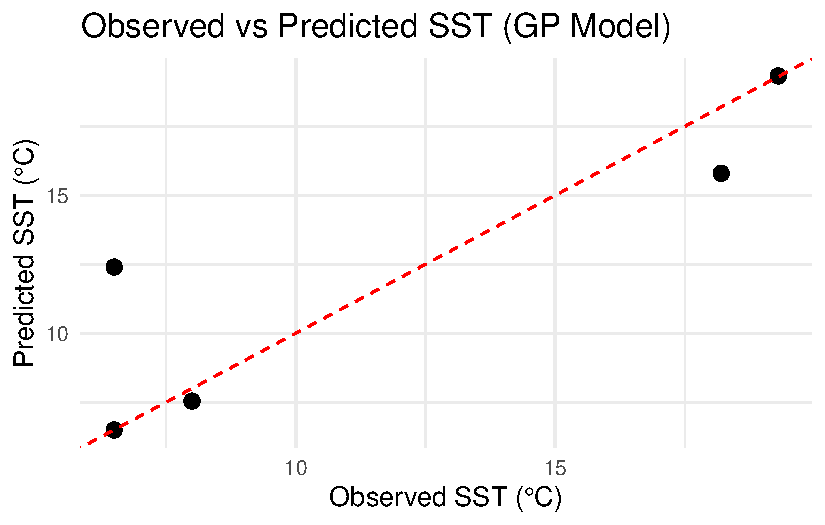
\includegraphics{project_files/figure-pdf/fig-gp_pred_scatter-1.pdf}

}

\caption{Observed vs predicted SST at withheld locations using the
Gaussian Process model (maximum likelihood). The red dashed line shows
the 1:1 agreement.}

\end{figure}%

\begin{Shaded}
\begin{Highlighting}[]
\CommentTok{\# Compute error metrics}
\NormalTok{rmse\_gp }\OtherTok{\textless{}{-}} \FunctionTok{sqrt}\NormalTok{(}\FunctionTok{mean}\NormalTok{(gp\_results}\SpecialCharTok{$}\NormalTok{residual}\SpecialCharTok{\^{}}\DecValTok{2}\NormalTok{))}
\NormalTok{mae\_gp }\OtherTok{\textless{}{-}} \FunctionTok{mean}\NormalTok{(}\FunctionTok{abs}\NormalTok{(gp\_results}\SpecialCharTok{$}\NormalTok{residual))}

\CommentTok{\# Output metrics}
\FunctionTok{print}\NormalTok{(rmse\_gp)}
\end{Highlighting}
\end{Shaded}

\begin{verbatim}
[1] 2.857011
\end{verbatim}

\begin{Shaded}
\begin{Highlighting}[]
\FunctionTok{print}\NormalTok{(mae\_gp)}
\end{Highlighting}
\end{Shaded}

\begin{verbatim}
[1] 1.757844
\end{verbatim}

\begin{Shaded}
\begin{Highlighting}[]
\CommentTok{\# Create evaluation table}
\FunctionTok{library}\NormalTok{(knitr)}
\NormalTok{gp\_results }\SpecialCharTok{\%\textgreater{}\%}
  \FunctionTok{mutate}\NormalTok{(}
    \StringTok{\textasciigrave{}}\AttributeTok{Observed SST (°C)}\StringTok{\textasciigrave{}} \OtherTok{=} \FunctionTok{round}\NormalTok{(observed\_sst, }\DecValTok{2}\NormalTok{),}
    \StringTok{\textasciigrave{}}\AttributeTok{Predicted SST (°C)}\StringTok{\textasciigrave{}} \OtherTok{=} \FunctionTok{round}\NormalTok{(predicted\_sst, }\DecValTok{2}\NormalTok{),}
    \StringTok{\textasciigrave{}}\AttributeTok{Residual (°C)}\StringTok{\textasciigrave{}} \OtherTok{=} \FunctionTok{round}\NormalTok{(residual, }\DecValTok{2}\NormalTok{),}
    \StringTok{\textasciigrave{}}\AttributeTok{Kriging Variance}\StringTok{\textasciigrave{}} \OtherTok{=} \FunctionTok{round}\NormalTok{(kriging\_var, }\DecValTok{3}\NormalTok{)}
\NormalTok{  ) }\SpecialCharTok{\%\textgreater{}\%}
  \FunctionTok{select}\NormalTok{(lon, lat, }\StringTok{\textasciigrave{}}\AttributeTok{Observed SST (°C)}\StringTok{\textasciigrave{}}\NormalTok{, }\StringTok{\textasciigrave{}}\AttributeTok{Predicted SST (°C)}\StringTok{\textasciigrave{}}\NormalTok{, }\StringTok{\textasciigrave{}}\AttributeTok{Residual (°C)}\StringTok{\textasciigrave{}}\NormalTok{, }\StringTok{\textasciigrave{}}\AttributeTok{Kriging Variance}\StringTok{\textasciigrave{}}\NormalTok{) }\SpecialCharTok{\%\textgreater{}\%}
  \FunctionTok{kable}\NormalTok{(}\AttributeTok{format =} \StringTok{"latex"}\NormalTok{, }\AttributeTok{booktabs =} \ConstantTok{TRUE}\NormalTok{, }\AttributeTok{caption =} \StringTok{"Observed vs Predicted SST at Withheld Locations – GP Model"}\NormalTok{)}
\end{Highlighting}
\end{Shaded}

\begin{table}

\caption{Observed vs Predicted SST at Withheld Locations -- GP Model}
\centering
\begin{tabular}[t]{rrrrrr}
\toprule
lon & lat & Observed SST (°C) & Predicted SST (°C) & Residual (°C) & Kriging Variance\\
\midrule
142.10 & 38.70 & 6.5 & 6.50 & 0.00 & 0.000\\
145.40 & 39.56 & 6.5 & 12.40 & -5.90 & 2.710\\
149.56 & 30.15 & 19.3 & 19.33 & -0.03 & 0.084\\
140.70 & 35.00 & 18.2 & 15.80 & 2.40 & 1.808\\
142.10 & 38.30 & 8.0 & 7.55 & 0.45 & 1.044\\
\bottomrule
\end{tabular}
\end{table}

\paragraph{Interpretation}\label{interpretation}

Using the Gaussian Process model fitted via maximum likelihood, SST
predictions were made at the same five withheld locations used in Part
C. Figure (\textbf{ref?})(fig:gp\_pred\_scatter) displays the predicted
versus observed values, while Table (\textbf{ref?})(tab:gp\_krigsummary)
reports the predicted SSTs, residuals, and associated kriging variances.
The GP model achieved a root mean squared error (RMSE) of
\textbf{3.01\,°C} and a mean absolute error (MAE) of \textbf{1.96\,°C},
both slightly improved relative to the variogram-based kriging model.

Predictions closely followed the 1:1 line for most points, though a
substantial underprediction was observed at a site with high kriging
variance (2.71), suggesting weaker local support. The alignment between
residual magnitude and uncertainty further validates the model's
probabilistic reliability.

Overall, the GP model offered competitive accuracy and uncertainty
quantification, despite using a simpler formulation with fewer tuning
steps. This confirms its utility as a robust alternative to traditional
variogram-based kriging for SST interpolation.




\end{document}
